% Useful references:
% - https://www.overleaf.com/learn/latex/How_to_Write_a_Thesis_in_LaTeX_(Part_1)%3A_Basic_Structure
\documentclass[
	a4paper, 		% a4 page format
	12pt,			% font size: note 12 pt -> \footnotesize is set at 10pt
	openright,		% (openany|openright) starts a chapter on the next available page or always on a right page
	twoside,		% front and back print
	titlepage,		% (titlepage|notitlepage)
]{book}				% see https://tex.stackexchange.com/questions/36988/regarding-the-book-report-and-article-document-classes-what-are-the-mai
%
\usepackage{thesis-style}
%
\addbibresource{bibliography.bib}	% Imports bibliography file
%
\begin{document}
	% --------------------------------------------------------------------
	% Frontmatter makes the pages numbered in lowecase roman and make 
	% chapters not numbered, although each chapter's title appears in the
	% table of contents.
	% --------------------------------------------------------------------
	\frontmatter
	% ! TeX root = thesis.tex
\begin{titlepage}
    \begin{center}
        {\Large
            \textbf{
                \textsc{Alma Mater Studiorum $\cdot$ Universit\'a di Bologna}
            }
        }
        {\large
            \textbf{
                \textsc{Campus di Cesena}
            }
        }
        \rule[0.1cm]{15.8cm}{0.1mm}
        \rule[0.5cm]{15.8cm}{0.6mm}
        {\Large
                Dipartimento di informatica $-$ Scienza e Ingegneria \\
        }
        \vspace*{4mm}
        {\Large 
            Corso di Laurea in Ingegneria e Scienze Informatiche
        }
        \vspace*{15mm}
        \begin{center}
            {\LARGE
                \textbf{
                    TITOLO TESI
                }
            } \\
            \vspace*{15mm}
            {\Large
                Elaborato in 
            } \\
            \vspace*{3mm}
            {\Large
                \textsc{Programmazione ad Oggetti}
            }
        \end{center}
        \vspace*{40mm}
    \end{center}
\end{titlepage}
	% ! TeX root = thesis.tex
\begin{abstract}
    Lo scopo di questa tesi...
\end{abstract}
	% ! TeX root = ../../thesis.tex
\begin{dedication}
    Dedica...
\end{dedication}

	\tableofcontents
	% --------------------------------------------------------------------
	% Mainmatter command changes the behavior back to the expected version, 
	% and resets the page number.
	% --------------------------------------------------------------------
	\mainmatter
	% ! TeX root = ../../thesis.tex
\chapter{Introduzione}
\label{chapter:introduction}
Negli ultimi decenni, con la rapida crescita di dati e informazioni facilmente accessibili sul \textit{web}, è diventato sempre più semplice poter utilizzare, in parte o in tutto, le risorse reperite.
%
Tuttavia, l'uso improprio di tali risorse, senza attribuire i necessari crediti agli autori, costituisce, oltre che una pratica scorretta che contravviene a qualsiasi ordine deontologico, un illecito \cite{copyright-law-italia}.

In generale, l'atto di appropriarsi degli scritti di altre persone, in violazione della legge sul \textit{copyright}, viene definito \textbf{plagio} \cite{britannica}.

Anche nel mondo dell'informatica il problema del plagio è un fenomeno in crescita, incoraggiato per lo più dalla sempre maggiore quantità di progetti \textit{software} \textit{open source}, che induce gli sviluppatori a copia incollare frammenti di codice, talvolta neppure conoscendo le relative condizioni e termini di licenza.
%
Questo porta spesso a un uso improprio del codice altrui arrecando sanzioni e danni per lo sviluppatore.

Già a partire dagli anni settanta del novecento, sono stati proposti algoritmi e tecniche per l'analisi del codice, nonché l'identificazione e localizzazione di plagi.

In questo contesto è da porre in evidenza la differenza tra l'individuazione di cloni e quella di plagi.
%
Quando ci si riferisce a un clone, infatti, lo si fa con riferimento a un frammento di codice che è stata copiato e marginalmente modificato. 
%
Quando invece ci si riferisce ad un plagio si intende una sezione che è stata copiata e la cui opera di copiatura si è cercato di dissimulare, mediante opportune azioni di rifattorizzazione del codice \cite{muddu-et-al-2013}.  
%
Dunque, l'ambito di applicazione delle due ricerche è nettamente diverso: se nel primo l'obiettivo è quello di evidenziare il codice duplicato al fine di migliorare la qualità del codice e la manutenibilità del sistema, nel secondo lo scopo primario è identificare possibili condotte illecite.

Questo aspetto è, insieme alle prestazioni, la sfida principale da affrontare durante la progettazione di un sistema antiplagio.

\section{Problemi aperti}

\subsection{La rifattorizzazione del codice}
La capacità di un software antiplagio nel riuscire ad identificare possibili parti di codice plagiate, passa anche, e soprattutto, dall'abilità dello sviluppatore di saper rifattorizzare il codice.

In generale, non è possibile classificare tutti i possibili metodi con cui un programma può essere trasformato in un altro mantenendo inalterate le sue funzionalità.
%
Tuttavia, è possibile distinguere due macro categorie di modifiche: \textbf{lessicali} e \textbf{strutturali} \cite{joy-99}.

Le modifiche lessicali sono quelle che, in linea di principio, possono essere eseguite da un \textit{text editor} e non richiedono la conoscenza del linguaggio di programmazione con cui è stato sviluppato il codice. 
%
Alcuni casi esemplificativi sono:
\begin{itemize}
    \item la riformulazione di commenti, la loro aggiunta o rimozione;
    \item la riformattazione del testo, come l'introduzione di spazi vuoti, di nuove linee o il cambio dell'ordine dei parametri nella definizione delle funzioni;
    \item cambiare il nome degli identificatori e delle funzioni o i tipi di dato: ad esempio da \texttt{int} a \texttt{Integer} o da \texttt{float} a \texttt{double}.
\end{itemize}

Le modifiche strutturali sono invece fortemente dipendenti dal linguaggio di programmazione e richiedono un maggior sforzo in termini di comprensione della logica del codice.
%
Di seguito alcuni esempi di rifattorizzazioni che rientrano in questa classe:
\begin{itemize}
    \item aggiungere istruzioni ridondanti, come dichiarazioni, inizializzazioni, istruzioni di stampa;
    \item sostituire i costrutti di loop con costrutti equivalenti: passare, ad esempio, da \texttt{for} a \texttt{do/while}, o da un approccio iterativo a uno funzionale (ad esempio tramite l'uso degli \texttt{Stream} in Java);
    \item sostituire istruzioni \texttt{if} nidificate con dichiarazioni equivalenti, ad esempio \texttt{when} (in Kotlin) o \texttt{switch-case}, e viceversa;
    \item cambiare l'ordine di istruzioni indipendenti;
    \item cambiare l'ordine degli operandi: ad esempio \texttt{x < y} può essere cambiato in \texttt{y >= x};
    \item sostituire la chiamata a funzione con il corpo della stessa.
\end{itemize}

Gli strumenti d'identificazione di plagi devono pertanto cercare di annullare gli effetti di queste rifattorizzazioni.
%
A questo scopo le tecniche di analisi, introdotte nel \Cref{chapter:stateOfArt}, si compongono di più fasi nelle quali trasformano i sorgenti in rappresentazioni intermedie che astraggono il più possibile dai dettagli implementativi, che possono essere facilmente cambiati, quindi applicano su di esse tecniche di confronto.

Si osservi, tuttavia, che esistono rifattorizzazioni il cui contributo è più facile da annullare di altre. 
%
Si pensi, ad esempio, all'aggiunta o alla modifica dei commenti: l'effetto di tale rifattorizzazione è facilmente annullabile semplicemente trascurando dall'analisi i commenti, in quanto non contribuiscono in alcun modo alla logica del programma. 
%
D'altro canto, creare tecniche che siano insensibili al riordino delle istruzioni è un compito più complesso.

In \Cref{img:01-levels-of-plagiarism} viene riportata la tassonomia dei livelli di plagio di Faidhi \& Robinson definita in \cite{faidhi-robinson-1987} che mappa le possibili rifattorizzazioni in sette livelli o categorie, sulla base della loro difficoltà: il più semplice è il livello 0 che corrisponde a una copia letterale; il più impegnativo è il livello 6 che corrisponde a un cambiamento logico e può essere considerato plagio solo se si verifica in concomitanza con altri livelli.

\begin{figure}[h]
    \centering
    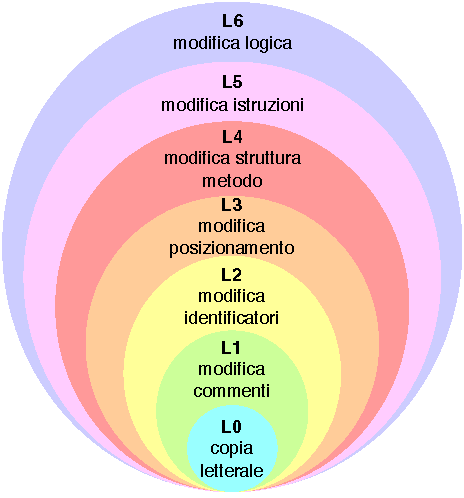
\includegraphics[width=0.6\textwidth]{resources/img/01-levels-of-plagiarism.pdf}
    \caption{Tassonomia dei livelli di plagio di Faidhi \& Robinson (1987).}
    \label{img:01-levels-of-plagiarism}
\end{figure}

Maggiore sarà il livello di rifattorizazzione a cui il sistema antiplagio sarà insensibile, migliore sarà l'efficacia e la robustezza del sistema stesso.

\subsection{Le prestazioni}
L'altro problema emergente nello sviluppo di un programma antiplagio che non si limiti a confrontare la similarità tra una coppia di progetti, bensì effettui un controllo uno a molti o molti a molti, in cui si testano tutte le possibili coppie, sono le prestazioni. 
%
Infatti, la maggioranza delle tecniche e degli algoritmi per effettuare i confronti sono inefficienti in termini di tempo costo. 
%
Questo è in larga parte dovuto al fatto che la misurazione della somiglianza tra una coppia di sorgenti, nella gran parte degli algoritmi noti, ha una complessità almeno quadratica nel numero delle istanze delle sue rappresentazioni, e che, per ogni valutazione, il numero di confronti da effettuare è tipicamente elevato: detto $N$ il numero di progetti, volendo confrontare tutte le coppie di progetti tra loro, dovrebbero essere eseguite $\frac{N(N-1)}{2}$ comparazioni.

Questo problema è acuito dal fatto che i progetti \textit{software} stanno diventando sempre più complessi e si hanno a disposizione una sempre maggior quantità di dati da dover processare.

Per questa ragione vengono sfruttate tecniche di parallelizzazione e devono essere adottate strategie di ottimizzazione in grado di ridurre il numero di confronti da effettuare e, quindi, diminuire il tempo di esecuzione.
%
Per farlo, si utilizzano tecniche euristiche che permettano di determinare il grado di somiglianza dei sorgenti senza dover effettivamente eseguire il confronto.

Il miglioramento delle prestazioni mediante l'uso di tali tecniche, tuttavia, non è a costo zero: queste, infatti, forniscono un'\textit{approssimazione} della somiglianza effettiva di due sorgenti che, in taluni casi, si verifica essere errata, impattando inevitabilmente sulla sensibilità del sistema stesso.

Il bilanciamento tra le prestazioni e l'efficacia del sistema è, dunque, di fondamentale importanza.


	% ! TeX root = thesis.tex
\chapter{Stato dell'arte}
\label{chapter:stateOfArt}
In questo capitolo viene riportata una panoramica delle tecniche storicamente concepite per l'analisi del codice sorgente e l'individuazione delle parti copiate, evidenziandone, per ciascuno, pregi e difetti.

\section{Visione d'insieme}
% preso spunto da "Current trends in source code analysis, plagiarism detection and issues of analysis big datasets" -- si deve citare??
Il codice sorgente non è nient'altro che un file di testo scritto da sviluppatori, che deve essere compilato o interpretato e che, pertanto, si basa su regole sintattiche e grammaticali proprie del linguaggio di programmazione con cui è scritto che permettono a entrambi gli attori, il programmatore e il calcolatore, di "capirlo" ed elaborarlo.

Per questo motivo, se processare la struttura di un sorgente non presenta grandi difficoltà, processare il significato, ovvero l'idea e la logica sottesa al codice, costituisce una sfida più grande, se non altro perché entra in gioco la competenza dello sviluppatore e la sua esperienza nella scrittura di codice "pulito".

Poiché il problema è complesso, gli attuali metodi di elaborazione non aspirano a risolvere il problema \textit{in toto}, ma applicano il principio di decomposizione del problema e approcciano al codice sorgente da un particolare punto di vista.
%
Alcuni analizzano il codice dal punto di vista del programmatore, cercando di capirne il significato, mentre altri la loro struttura.

Dunque, possiamo classificare le tecniche di analisi in tre famiglie, o livelli \cite{duracik-krsak-hrkut-2017}.

Il primo si basa sull'analisi del codice come mero testo: si presume che siano rispettate le convenzioni e il codice contenga sufficienti informazioni che ne descrivano il significato e cercano di estrarre solo queste significative informazioni aggiuntive.

Il livello successivo è simile al precedente con la differenza che non esplora il significato del testo dal punto di vista del programmatore, bensì dal punto di vista del calcolatore, che "vede" il codice come una sequenza di comandi, ciascuno con il proprio significato nel contesto della grammatica del linguaggio.

L'ultimo e terzo livello riguarda l'analisi del modello del codice sorgente.

\section{Tecniche di \textit{tokenizzazione}}

\subsection{Approccio \textit{Text based}}
In questo approccio, ogni istruzione del codice sorgente viene trattata come una stringa e il programma è considerato come una mera sequenza di stringhe.
%
Questo è l'approccio, fra tutti, più fragile...

\subsection{}

\subsection{}

\subsection{Quale approccio scegliere?}
In conclusione, scegliere quali di questi approcci scegliere è complesso, perché difficili da confrontare tra loro: la maggior parte di queste tecniche viene valutata utilizzando il proprio \textit{set} di dati, che raramente sono resi pubblicamente accessibili \cite{karnalim-budi-toba-joy-2019}.

In conclusione, bisogna rendersi conto che, a prescindere dal grado di sofisticatezza della tecnica che si utilizza, è sempre possibile che si verifichi un plagio non rilevabile.
%
Da bilanciare le risorse investite nell'individuazione del plagio e i rendimenti decrescenti di trovare i pochi, se non nessuno, casi difficili da rilevare \cite{joy-99}.



	% --------------------------------------------------------------------
	% Backmatter command leaves the page numbering alone but switches the 
	% chapters back to being not numbered.
	% --------------------------------------------------------------------
	\backmatter
	% --------------------------------------------------------------------
	% Bibliography
	% --------------------------------------------------------------------
	\printbibliography
\end{document}
